\section{Theorie}

\textbf{\underline{Ziel:}}
In diesem Versuch sollen die Leerlaufspannung und der Innenwiderstand verschiedener Spannungsquellen bestimmt werden.
\\
\\
Ist an einer Spannungsquelle kein Stromkreis angeschlossen, so ist in dieser eine Spannung $U_\text{0}$ messbar.
Wird jedoch ein Stromkreis angeschlossen, so ist die messbare Spannung $U$ kleiner als $U_\text{0}$.
Dies lässt sich mit der zweiten Kirchhof'schen Regel, der Maschenregel, begründen.
Diese besagt, dass die Summe aller Spannungen in einer Masche gleich $0$ ist:
\begin{equation}
\sum\limits_{i}^{n}U_i=0  .
\end{equation}
Für einen einfachen Stromkreis, wie in Abbildung \ref{fig:esk}, gilt mit $U=R\cdot I$ :
\begin{align}
  U_\text{0}&=\left(R_\text{i}+R_\text{a}\right) \cdot I \\
  \text{bzw.}\,\, U_\text{k}&=U_\text{0}-I\cdot R_\text{i} \label{eq:how}
\end{align}
Dabei ist $R_\text{i}$ der Innenwiderstand und $R_\text{a}$ der Lastwiderstand.
Die Spannung $U_\text{k}$ ist hier die Klemmenspannung und kann an der belasteten Quelle abgegriffen werden.
\begin{figure}[H]
  \centering
  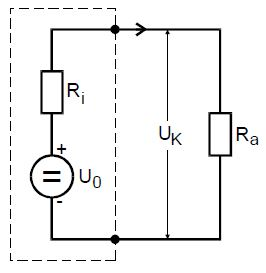
\includegraphics{text/Bilder/esk.jpg}
  \caption{Einfacher Stromkreis \cite[213]{sample}}
  \label{fig:esk}
\end{figure}
Da bei einem hochohmigen Widerstand sehr wenig Strom fließt, lässt sich Gleichung \eqref{eq:how} wie folgt nähern:
\begin{equation}
  U_\text{k} \approx U_\text{0}
\end{equation}
Da der Strom bei anderen Spannungsquellen nicht zwingend konstant fließen muss, muss in manchen Fällen mit
der diffentiellen Stromstärke gerechnet werden.
Der im System vorhandene Innenwiderstand $R_\text{i}$ beeinflusst ebenfalls die elektrische Leistung $N$.
Aufgrund von $R_\text{i}$ lässt sich keine beliebig hohe Leistung erreichen und es gilt:
\begin{equation}
  N=I^2 \cdot R_\text{a}=\frac{U^2_\text{0}}{(R_\text{i}+R_\text{a})^2}R_\text{a} .
  \label{eqn:leistung}
\end{equation}
Die Funktion wird bei $R_\text{i}=R_\text{a}$ maximal. In diesem Fall wird von Leistungsanpassung gesprochen.
